%!TEX root = ../proteoform_suite_manual.tex
%---------------------------------------------------------------------
%	RAW EXPERIMENTAL COMPONENTS
%---------------------------------------------------------------------

\section{Raw Experimental Components}


\subsection{Overview}

On this page, raw experimental components are read in from the file(s) loaded under Deconvolution Results for Identification and Deconvolution Results for Quantification on the Load Results page. A raw experimental component is an individual proteoform observation as reported in the deconvolution results file(s). 

\subsection{Run Page}
\begin{itemize}
\item Load the deconvolution results file(s) on the Load Results page under Deconvolution Results for Identification. If desired, label the biological replicate, fraction, technical replicate, and condition for each file (see \textbf{Load Results} section)
\item If performing a quantitative analysis, load the deconvolution results file(s) on the Load Results page under Deconvolution Results for Quantification. Label the biological replicate, fraction, technical replicate, and condition for each file (see \textbf{Load Results} section)
\item Set all parameters as desired for current analysis (see below)
\item Click Run Page button (top right)
\end{itemize}

\subsection{Set Parameters}
\begin{figure}[h]
\centering
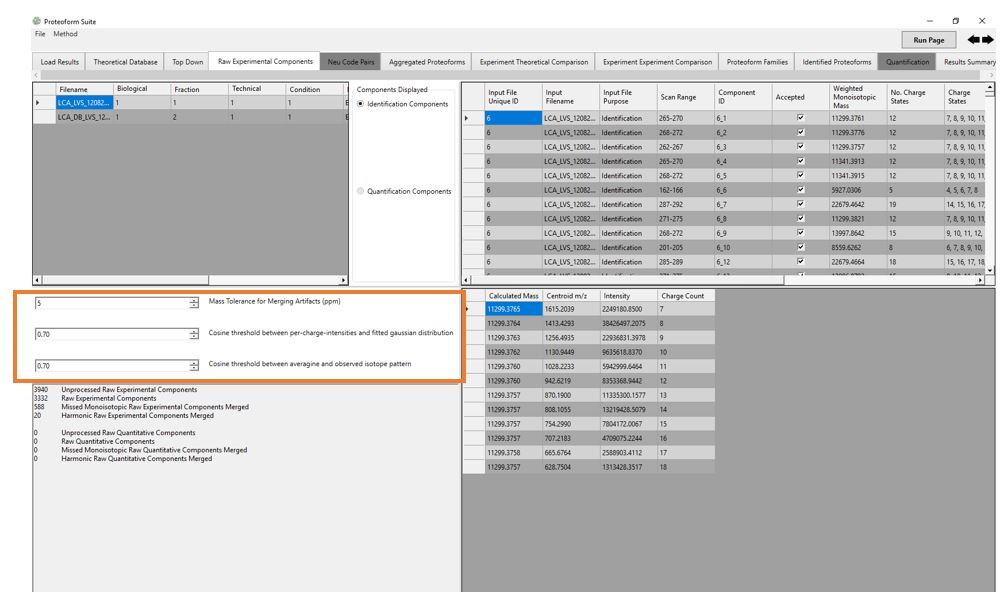
\includegraphics[scale=0.5]{figures/rawcomponents1.jpg}
\end{figure}
\begin{itemize}
\item Mass tolerance for Merging Artifacts (ppm): mass tolerance used to merge deconvolution artifacts including missed monoisotopic mass differences and charge state harmonics
\item Cosine threshold between per-charge intensities and fitted gaussian distribution: minimum value as described for FLASHDeconv deconvolution results
\item Cosine threshold between averagine and observed isotope pattern: minimum value as described for FLASHDeconv deconvolution results
\end{itemize}
\subsection{Results}
\begin{itemize}
	\item Unprocessed Raw Experimental Components: the number of raw experimental components for identification before merging artifacts
	\item Raw Experimental Components: the number of raw experimental components for identification after merging artifacts
	\item Missed Monoisotopic Raw Experimental Components Merged: the number of raw experimental components for identification artifacts merged due to being missed monoisotopic errors within the set mass tolerance
	\item Harmonic Raw Experimental Components Merged: the number of raw experimental components for identification artifacts merged due to being charge state harmonic errors within the set mass tolerance
	\item Unprocessed Raw Quantitative Components: the number of raw experimental components for quantification before merging artifacts
	\item Raw Quantitative Components: the number of raw experimental components for quantification after merging artifacts
	\item Missed Monoisotopic Raw Quantitative Components Merged: the number of raw experimental components for quantification artifacts merged due to being missed monoisotopic errors within the set mass tolerance
	\item Harmonic Raw Quantitative Components Merged: the number of raw experimental components for quantification artifacts merged due to being charge state harmonic errors within the set mass tolerance
	\begin{figure}[h]
\centering
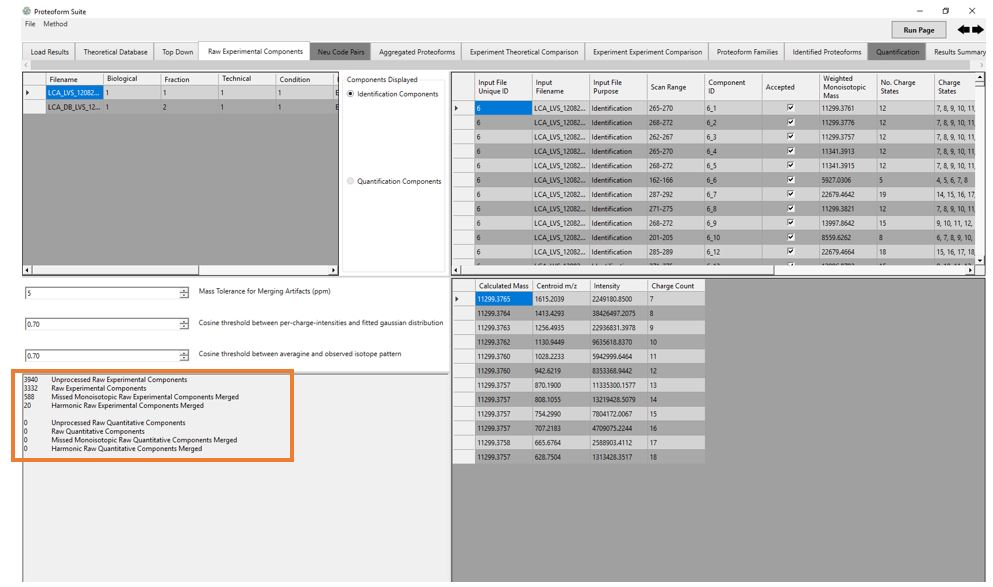
\includegraphics[scale=0.5]{figures/rawcomponents2.jpg}
\end{figure}
\pagebreak
	\item Raw Experimental Components table: the top right table displays raw experimental components for either Identification or Quantification (depending on selection of Components Displayed to the left of the table)
		\begin{figure}[h]
\centering
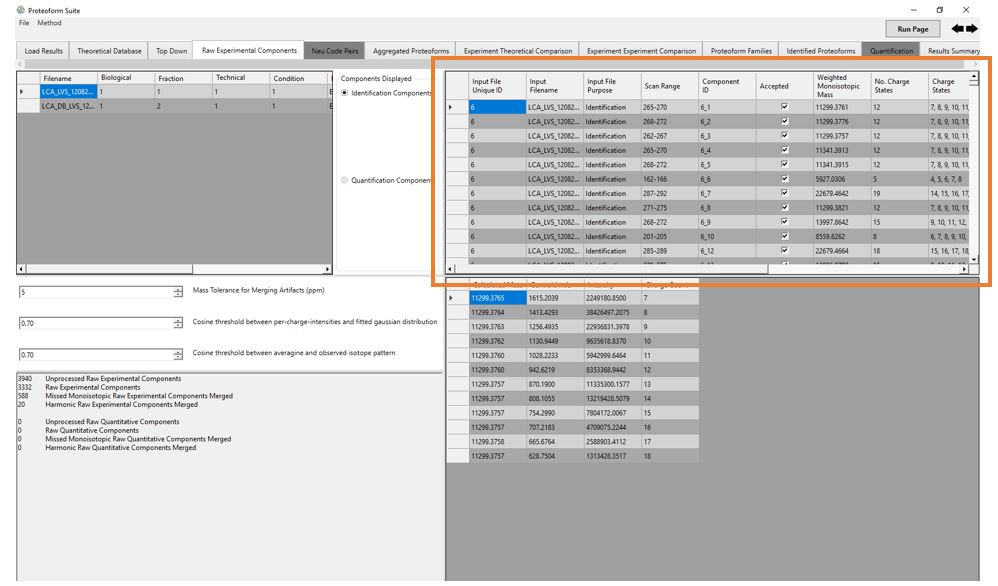
\includegraphics[scale=0.5]{figures/rawcomponents3.jpg}
\end{figure}
	\begin{itemize}
		\item Input File Unique ID: file ID number for filename of Deconvolution Results for Identification or Quantification for this raw experimental component
		\item Input Filename: filename of Deconvolution Results for Identification or Quantification for this raw experimental component
		\item Input File Purpose: either Identification or Quantification
		\item Scan Range: MS scan range for this raw experimental component
		\item Component ID: Proteoform Suite given ID for this raw experimental component; file ID\_component \#
		\item Accepted: checked if this raw experimental component is accepted for analysis
		\item Weighted Monoisotopic Mass: monoisotopic mass of raw experimental component weighted by intensity of each charge state (more intense charge states are higher weighted)
		\item No. Charges: number of charge states for this raw experimental component
		\item Charge States: comma-separated list of charge states for this raw experimental component
		\item Intensity Sum: intensity of this raw experimental component, charge state normalized
		\item RT Range: retention time range
		\item Apex RT: apex retention time as reported
		\item Reported Monoisotopic Mass: monoisotopic mass reported by deconvolution input
		\item Reported Intensity: intensity reported by deconvolution input
	\end{itemize}
	\item Charge States table: the bottom right table displays all charge states from the raw experimental component selected in the Raw Experimental Components table (top right)
		\begin{figure}[h]
\centering
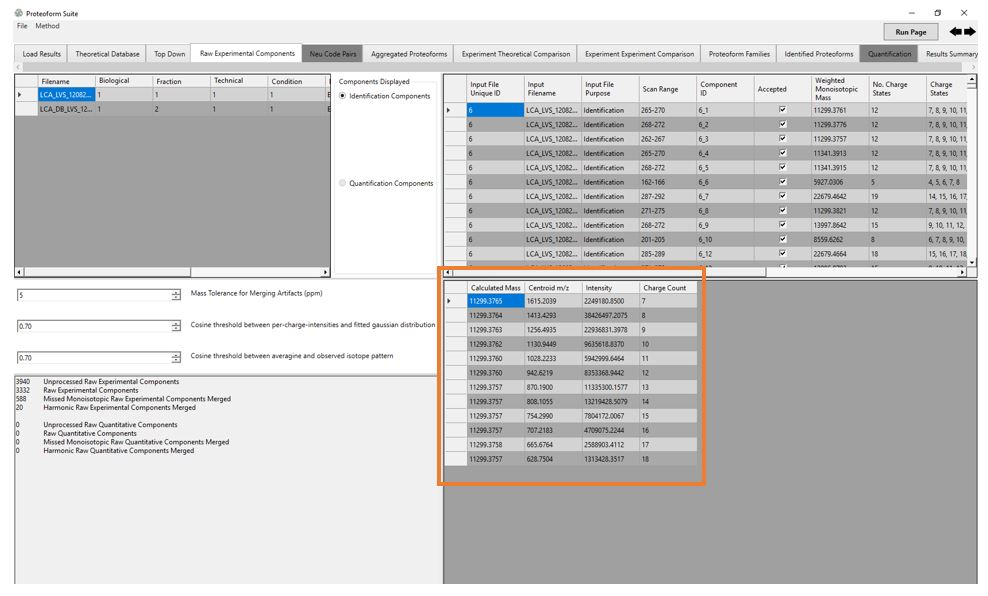
\includegraphics[scale=0.5]{figures/rawcomponents4.jpg}
\end{figure}
	\begin{itemize}
		\item Calculated Mass: monoisotopic mass of this charge state
		\item Centroid m/z: monoisotopic \textit{m/z} value of this charge state
		\item Intensity: charge normalized intensity of this charge state
		\item Charge count: number of this charge state
	\end{itemize}
\end{itemize}